\documentclass{article}




\usepackage[english,american]{babel}
\usepackage{titling}
\usepackage{lipsum}
\usepackage{booktabs}
\usepackage[table,xcdraw]{xcolor}
\usepackage{float}
\usepackage{changepage}
\usepackage{geometry}
\usepackage{graphicx}


\geometry{total={210mm,297mm},
	left=25mm,right=25mm,%
	bindingoffset=0mm, top=20mm,bottom=20mm}

\pretitle{\begin{center}\Huge\bfseries}
\posttitle{\par\end{center}\vskip 0.5em}
\preauthor{\begin{center}\Large\ttfamily}
\postauthor{\end{center}}
\predate{\par\large\centering}
\postdate{\par}

\author{Adam Lieberman, Ravish Chawla, \& Garrett Mallory}
\date{March 5, 2017}
\title{Project Proposal}

\begin{document}
  
\maketitle
\begin{abstract}
    When a patient enters a clinical setting, notes are written down to help better diagnose a patient based off their symptoms, lab results, and surgical notes. Diagnoses are not always correct and in a clinical setting, an increase in confidence of a diagnosis is always welcome. We aim to create a system that, once developed and deployed, leverages large patient-based datasets to confirm that a doctor prescribed diagnosis, in the form of an ICD-9 code, is accurately based upon clinical observations. This system delivers a few main advantages: (1) Our algorithm can review thousands of clinical notes and diagnose a patient before a doctor can review and diagnose a single patient (2) Our model can constantly take in new data and be updated to achieve more accurate diagnoses (3) The system can serve as a second look for a doctor who has a prescription in mind. 

In this proposal, we discuss the characteristics of the data we aim to examine, the processing pipeline for this data, an overview of some features we plan to engineer, deep learning algorithms we plan to explore, architecture for our system, and a cost-benefit analysis of the end product. 
\end{abstract}


\section{High-level Approach}
We are creating a deep learning system called Dr. ANN that will take in a clinical note and output a predicted diagnosis in the form on an ICD-9 code. Throughout the development process we will explore a variety of feature representations such as bag-of-words, word-to-vec, and tfidf. We will explore deep learning algorithms such as artifical neural networks, end-to-end memory networks, and long short term memory. We aim to use the power of deep learning to accurately recommend diagnoses based off of a patient's clinical note.

\section{Today's Diagnosis}
Today, doctors are manually diagnosing patients. Handwritten/digital clinical notes are being observed and doctors are using their best judgment to accurately diagnose said given patient. Doctors are specialized and hence have great knowledge of the medical field to diagnose patients. There has been a great deal of research on using deep learning, particularly on Recurrent Neural Networks and Long Short Term Memory, to diagnose patients, but no system has been deployed in a hospital or doctor's office. This is partly due to machine error. Computers are not perfect and do make mistakes. Diagnosing a patient can be a life-threatening event and to put this fate in a computer's hands can be quite dangerous. However, a computer trained to recommend diagnoses like a doctor can serve as a second-look for the doctor. The deep learning algorithm could potentially discover diagnoses the doctor never thought about and could be a great point of reference to assist the doctor in diagnosing patients.

\section{Our Approach}
We aim to use deep learning to essentially train a computer system to make recommendations of diagnoses at a degree that a doctor can.  We are training a deep network to think like a doctor. With or system doctors will be able to input their clinical notes and the note will be run through our deep learning algorithm. A predicted ICD-9 code will then be returned to the doctor to help assist in diagnosing a patient. Additionally, our system can predict thousands of diagnosis recommendations before a doctor can read a clinical note and make one recommendation. This can save the doctor time as calling alternate doctors for a few second opinions is a slow process.Our system will allow doctors to confirm or validate their hypothesis for a given patient. Additionally, a patient could use our system to self-diagnose themselves prior to visiting a doctor's office. They could then research their diagnosis and have a better perspective on their current condition. 

\section{Risks \& Rewards}
There are associated risks with what we are aiming to achieve. Deep learning has shown to provide great learning results, but there is a chance that our models perform poorly. This could be a result from not having enough data or not finding the optimal parameters for our model. Neural networks are notoriously difficult to evaluate and machine learning in general is not always understood as a trusted tool. This would render our product useless to doctors and patients as it would not provide accurate diagnoses. However, if we are successful we could greatly assist doctors in providing diagnosis recommendations. This system could be utilized in many hospitals and intensive care units and could potentially accurately diagnose thousands of patients in seconds. 

\section{Data}
We will be utilizing data from MIMIC-III, a large publicly-available database comprising of de-identified health-related data associated with approximately 60,000 patients from the critical care units of Beth Israel Deaconess Medical Center from 2001 to 2012. The database is comprised of static and dynamic data ranging from birth dates to demographics to laboratory test results to diagnoses to imaging reports to clinical notes. For our purposes we will be analyzing clinical notes and predicting associated diagnoses. Thus, we will particularly make use of the following tables: 

\begin{itemize}
\item diagnoses\_icd
\item noteevents
\end{itemize}

\noindent The diagnoses\_icd table contains patient diagnoses. The noteevents contains the following type of clinical notes: 
\begin{itemize}
\item Discharge Summary - A summary written by the physician (or possibly a team of physicians) at the time of discharge from the ICU.
\item Radiology reports - Reports from imaging procedures such as MRI, CT, and Ultrasounds.
\item Nursing progress reports - Daily notes from the nursing staff.
\end{itemize}

\noindent For our purposes, we will use all three types of notes, grouped by individual patients. Along with these notes, we will use other features such as the diagnostic date, lab result values, and other information that can be extracted. We will clean the data and these features will be fed into our Neural Network, which will retrieve the best set of features. We will also handle cases in which a patient may have notes from multiple visits, by grouping the events together to obtain a result based on all data available for the user within the observation window.
\section{Feature Construction}
To pass our clinical text data into our deep learning algorithm we will need to construct features. We will explore the following features: 
\begin{itemize}
\item \textbf{Bag-of-words}:  The bag of words model is a representation used in natural language processing. With this model, a text such as a sentence or document is represented as a bag of its words where grammar and word order are disregarded. After the text is transformed into the bag of words, we can calculate various measures to characterize the text. For instance, we can look at the term frequency. This is the number of times a term appears in our text. We can construct this text vector and use this feature  in our deep learning algorithms.
\item \textbf{Word2vec} -  We can build  word projections in a latent space of $N$ dimensions where $N$ is the size of the word vectors obtained. The vector will contain float values that represent the coordinates of the words in this $N$ dimensional space. This allows us to view our text vector in a different and continuous dimension space, which may attribute to different and more interesting calculus characteristics. 
\item \textbf{Term Frequency-Inverse Document Frequency (TFIDF)} - TFIDF allows us to reflect how important a word is to a document in a corpus. Some words are very frequent like "the", "a", "is", but carry very little meaningful information about the actual content of the document. If we were to look at a frequency count in a document that has many of these non-meaningful words our model might perform worse as it is not giving importance to the rarer yet more interesting terms.  We can re-weight the count features and use this feature vector in our deep learning algorithm. 
\end{itemize}

\section{Deep Learning Architecture}
After obtaining the preprocessed features from the clinical notes, we will train a Neural Network in order to find a model that can best predict diagnostic codes. Input to the Neural Network will consist of separated words from the clinical notes, and features generated from TfIDF. Instead of predicting ICD-9 codes to the full precision, our model will be trained to predict only up to first 3 digits, limiting the number of classes substantially. Higher precision codes will be predicted using a separate model. We will be using this approach because the large amount of ICD-9 codes may limit the number of training examples the model will have available to train on for a specific class. For instance, there might be few patients with ICD-9 code 250.6, Diabetes with neurological manifestations. However, the number of patients with Diabetes, and an ICD-9 code of type 250.*, may be much higher.  We are planning to analyze and research the following deep learning models: 
\begin{itemize}
\item \textbf{Basic Artificial Neutral Network}:
\item \textbf{End to End Memory Network}:
\item \textbf{Long Short Term Memory}:
\end{itemize}


\section{Performance Measurements}

\section{Web Application}
Once our deep learning algorithm has been finely tuned, it is ready for predictions. To make our system user friendly, we are creating a python-backed web application where doctors and patients can input their clinical record and view the model's predicted diagnoses. In our system, they will find information regarding the top 3 predicted diagnoses and sample clinical reports for each predicted diagnosis. This will allow them to evaluate and gain insight into the condition. The web application architecture is as follows: 
\begin{itemize}
\item \textbf{Frontend} - The frontend will consist of HTML, CSS, Javascript, and JQuery. 
\item \textbf{Backend} - The backend deep learning results and web scraping for ICD-9 code descriptions will be performed with python.
\item \textbf{Microframework} - To connect the frontend and backend together we will use the flask microframework. We will make use of Jinja2 to pass some backend python data to the HTML template on the frontend so that it is viewable for users. 
\end{itemize}

We have started the UI/UX process and have built the base of our frontend: 

\begin{figure}[H]
\begin{center}
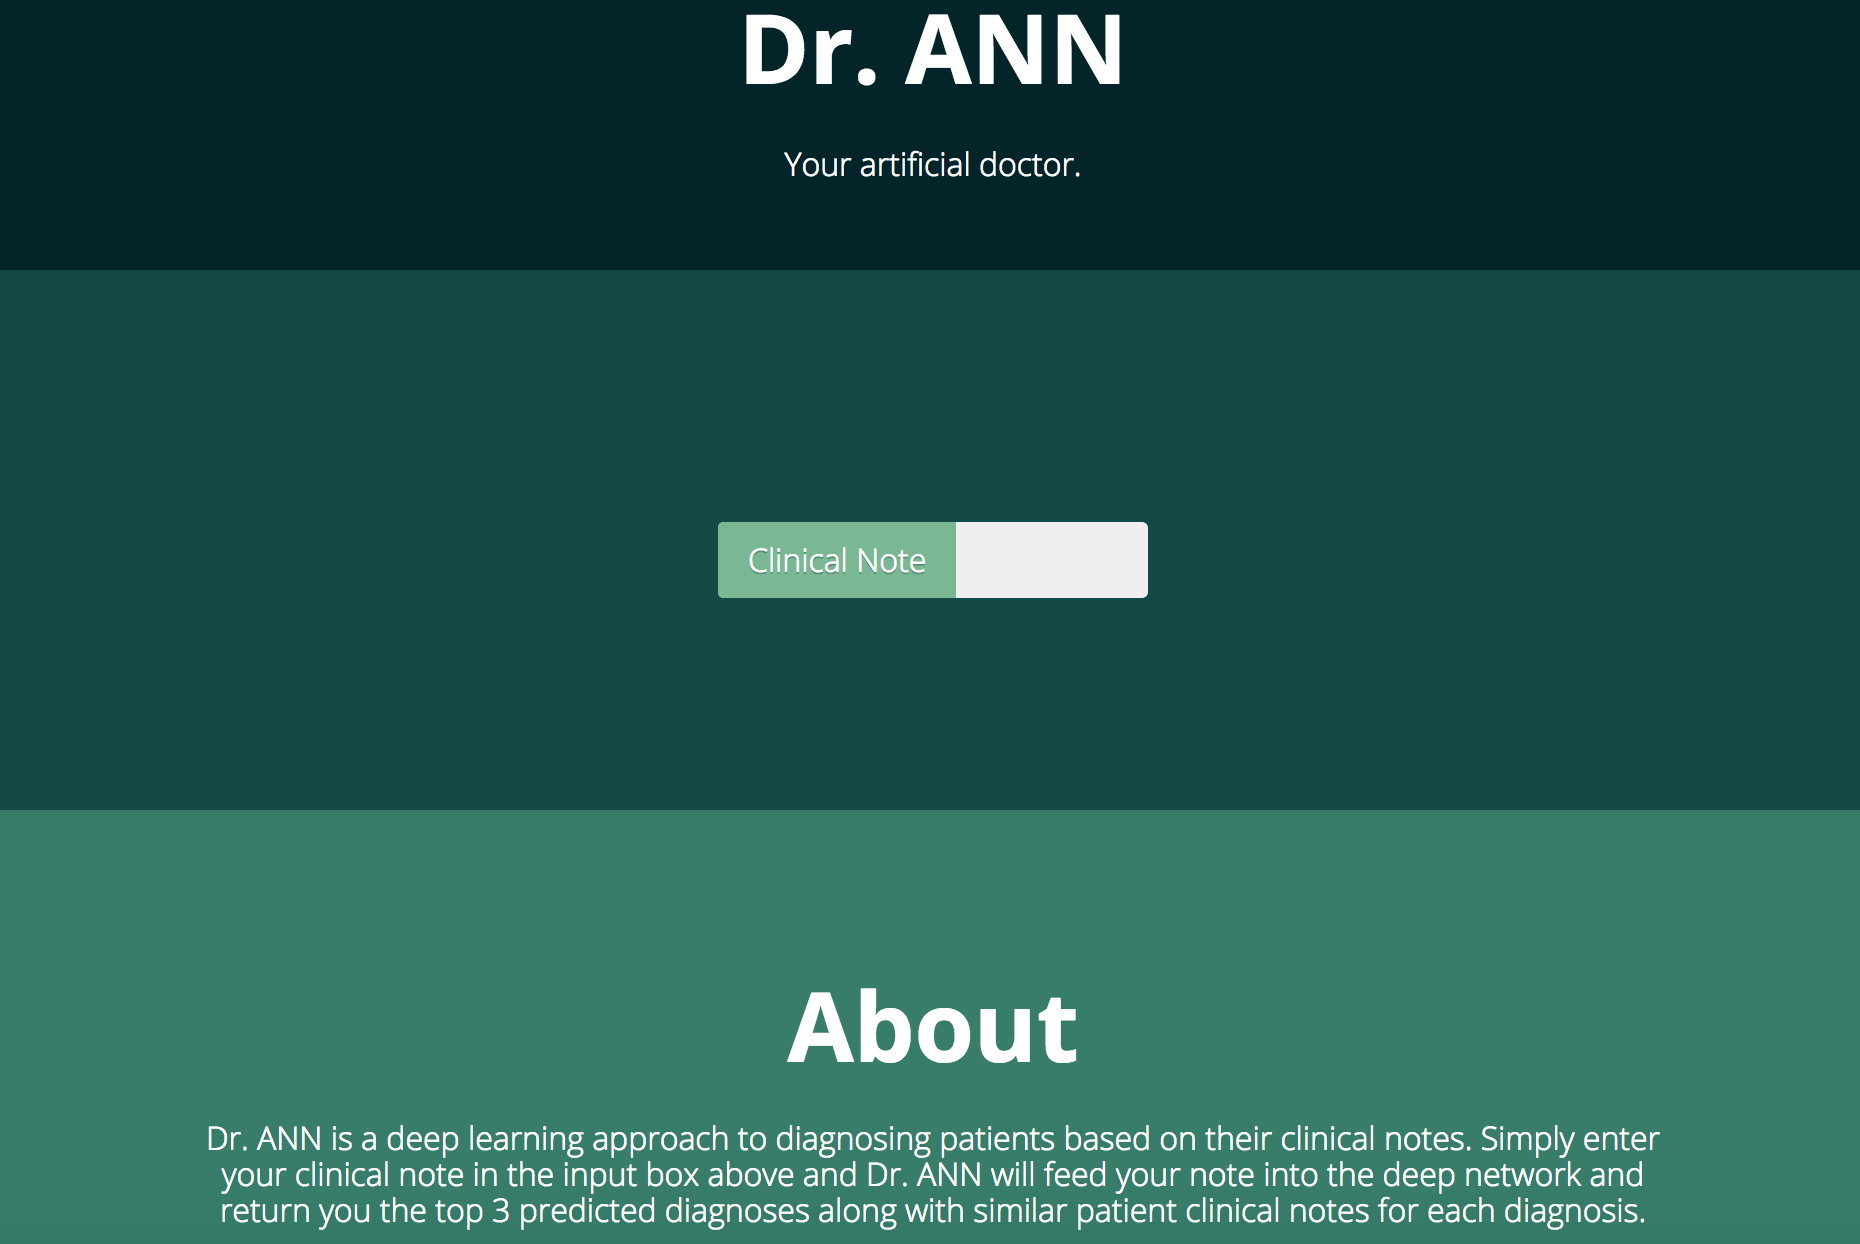
\includegraphics[width=300px,height=200px]{input.png}
\caption{Homepage to enter in clinical note}
\end{center}
\end{figure}

\noindent The above image displays the homepage for Dr. ANN. Here, doctors and patients can enter in a clinical note in the input field and submit it to the deep learning algorithm. 

\begin{figure}[H]
\begin{center}
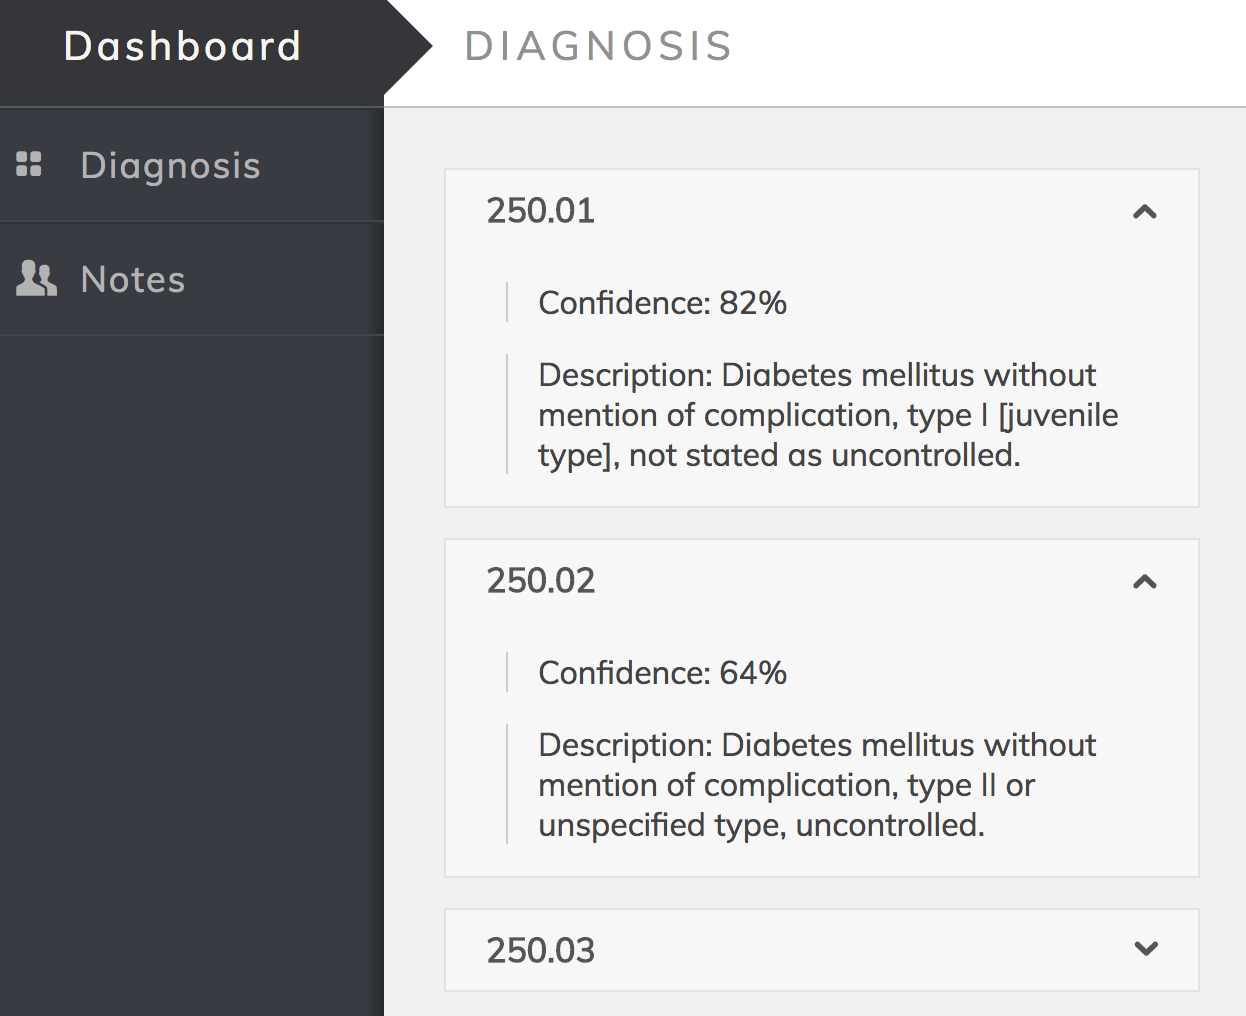
\includegraphics[width=300px, height=200px]{diagnosis.png}
\caption{Diagnoses tab in user dashboard}
\end{center}
\end{figure}

\noindent Above we have the user dashboard on the diagnosis page. Here the user can see the top 3 returned diagnoses in the form of an ICD-9 code from the deep learning algorithm.  If the drop down is clicked on the ICD-9 code box, the user can see the confidence from the deep learning algorithm for the particular predicted diagnosis as well as information about the diagnosis. 

\begin{figure}[H]
\begin{center}
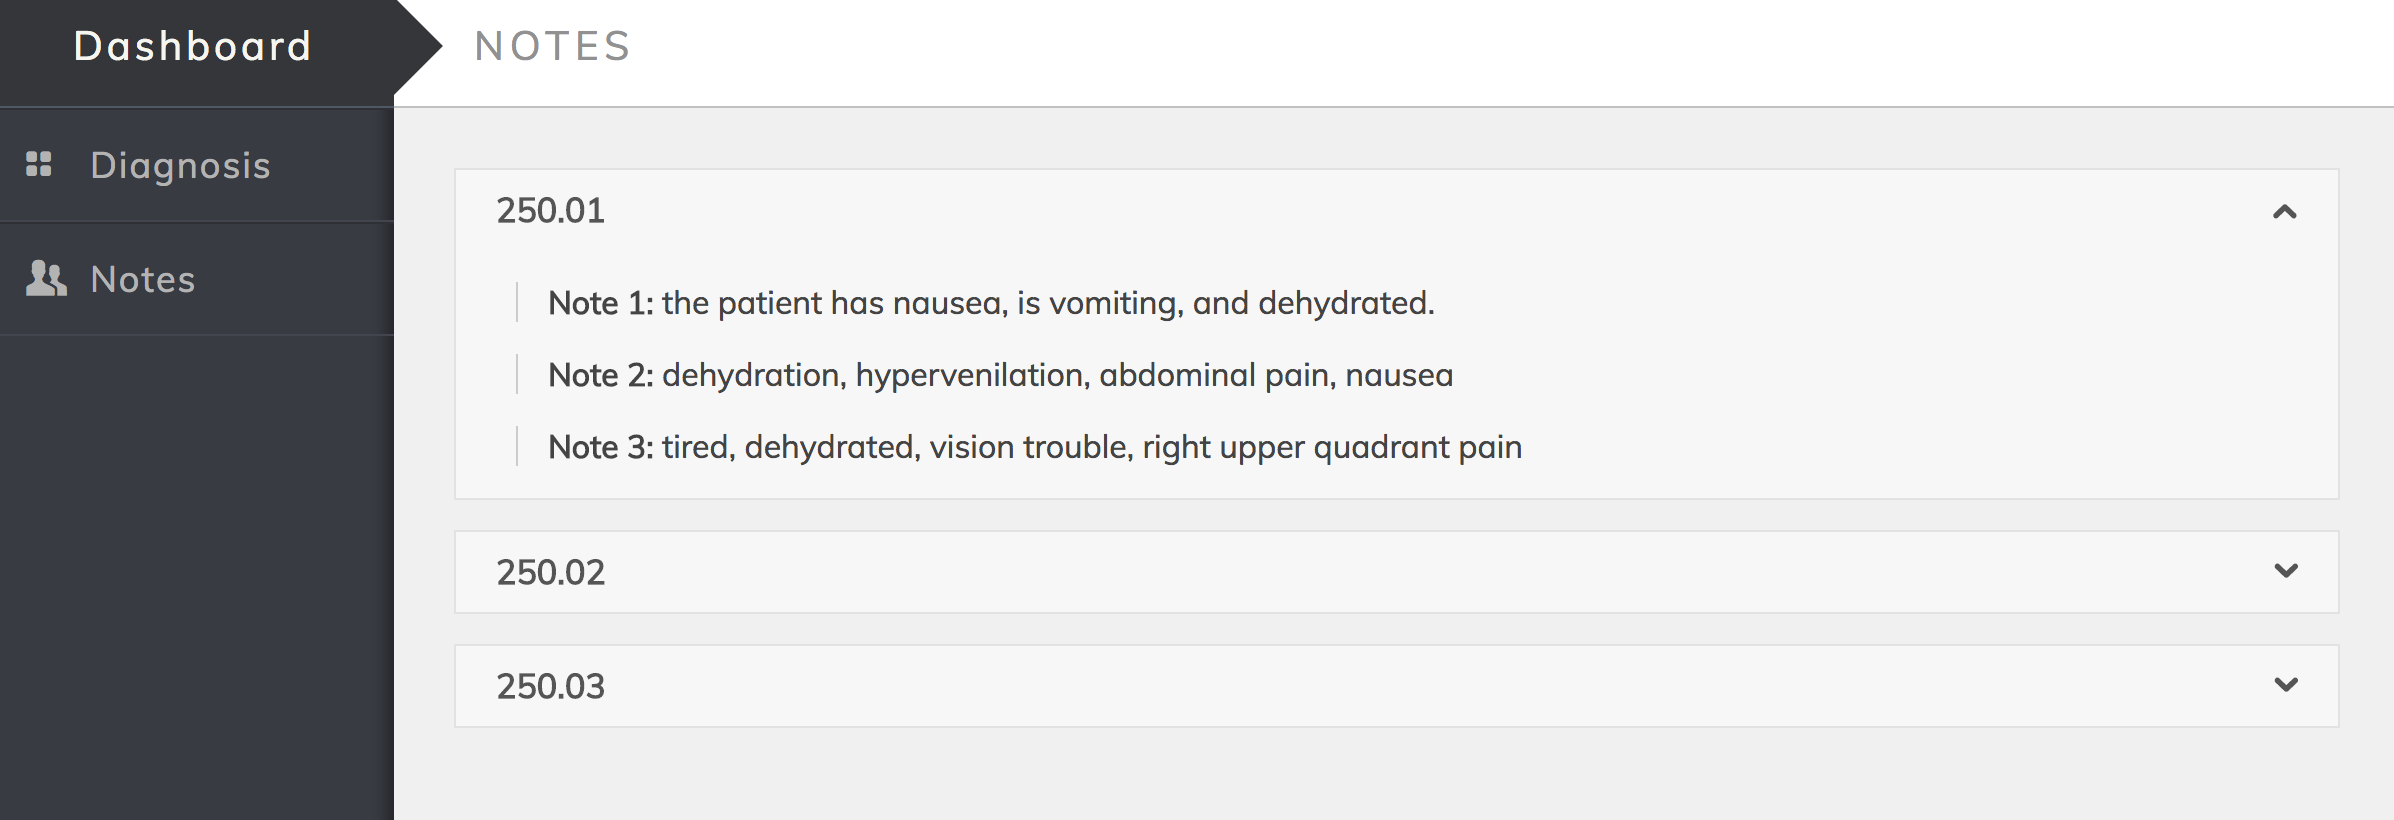
\includegraphics[width=\textwidth, height=200px]{notes_sample.png}
\caption{notes tab in user dashboard}
\end{center}
\end{figure}

\noindent Above we see that dashboard  on the notes tab. Here the user can see sample clinical notes for the diagnosis. This can better help the user identify if the diagnosis prediction is related to the patient conditions. 

\section{Cost}
The table below displays the cost for each aspect of our project:
% Please add the following required packages to your document preamble:
% \usepackage[table,xcdraw]{xcolor}
% If you use beamer only pass "xcolor=table" option, i.e. \documentclass[xcolor=table]{beamer}
\begin{table}[H]
\centering
\label{my-label}
\begin{tabular}{llll}
\rowcolor[HTML]{4674C1} 
{\color[HTML]{FFFFFF} Task}                                                                                                      & {\color[HTML]{FFFFFF} Time Estimate} & {\color[HTML]{FFFFFF} Rate} & {\color[HTML]{FFFFFF} Cost} \\ \hline
\hline
\rowcolor[HTML]{D8E1F1} 
Frontend Application Development                                                                                                 & 12 hours                             & \$45/hr                     & \$540.00                    \\
\begin{tabular}[c]{@{}l@{}}Backend: Deep Learning Algorithm\\                 (Parameter Tuning, Model Exploration)\end{tabular} & 20 hours                             & \$125/hr                    & \$2500.00                   \\
\rowcolor[HTML]{D8E1F1} 
Backend: Preprocessing                                                                                                           & 3 hours                              & \$60/hr                     & \$180.00                    \\
Backend: Feature Engineering                                                                                                     & 3 hours                              & \$60/hr                     & \$180.00                    \\
\rowcolor[HTML]{D8E1F1} 
Backend: Data Scraping for FrontEnd Delivery                                                                                     & 1 hour                               & \$50/hr                     & \$50.00                     \\
Resource: M4.XLarge AWS Instance                                                                                                 & 10 hours                             & \$0.215/hr                  & \$2.15                      \\
\rowcolor[HTML]{D8E1F1} 
Resource: P2 AWS Instance                                                                                                        & 25 hours                             & \$0.90/hr                   & \$22.50                     \\ \hline
\hline
Total Estimate:                                                                                                                  & 39 hours                             &                             & \textbf{\$3474.65}                  
\end{tabular}
\caption{Labor Cost}
\end{table}
The hourly rates were averaged from various freelance development sources.

\section{Timeline}



\section{Literature Survey}

\section{References}
\end{document}